\chapter{Results and Discussions}
\section{User Interface Representation}
In order to make user interface, many controls are used. Some of which are as follow:
\begin{enumerate}
\item \textbf{\emph{TextView:}}\\
Text View displays text to the user and optionally allows them to edit it. A TextView is a complete text editor, however the basic class is configured to not allow editing.

\item \textbf{\emph{EditText:}}\\
EditText is a thin veneer over TextView that configures itself to be editable. 
\item \textbf{\emph{Button:}}\\
A button consists of text or an icon (or both text and an icon) that communicates what action occurs when the user touches it.

\item \textbf{\emph{List View:}}\\
ListView is a view group that displays a list of scrollable items. The list items are automatically inserted to the list using an Adapter that pulls content from a source such as an array or database query and converts each item result into a view that's placed into the list.

\item \textbf{\emph{Check Boxes:}}\\
Checkbox is a control or widget that can be activated with a finger touch and can be polled in the application's code for
a checked and uncheckked state.

\end{enumerate}
\subsection{Brief Description of Various Modules}
\subsubsection{GCM Messaging}
Google Cloud Messaging for Android (GCM) is a service that allows you to send data from your server to your users' Android-powered device, and also to receive messages from devices on the same connection. The GCM service handles all aspects of queueing of messages and delivery to the target Android application running on the target device. GCM is completely free no matter how big your messaging needs are, and there are no quotas.

\textbf{\emph{GCM Working}}
\begin{enumerate}
\item Android device sends SENDER\_ID to GCM Server for registration.
\item After successful registration, GCM sends Registration ID to Android device.
\item After getting registration id, Android device sends registration id to Web Server.
\item Store registration id in our database at the server.
\item Whenever Push Notification needed, get registration ids from server, and send the request to GCM with registration id and message.
\item After push notification request, GCM sends Push Notifications to Android device.
\end{enumerate}

\begin{figure}[H]
\centering 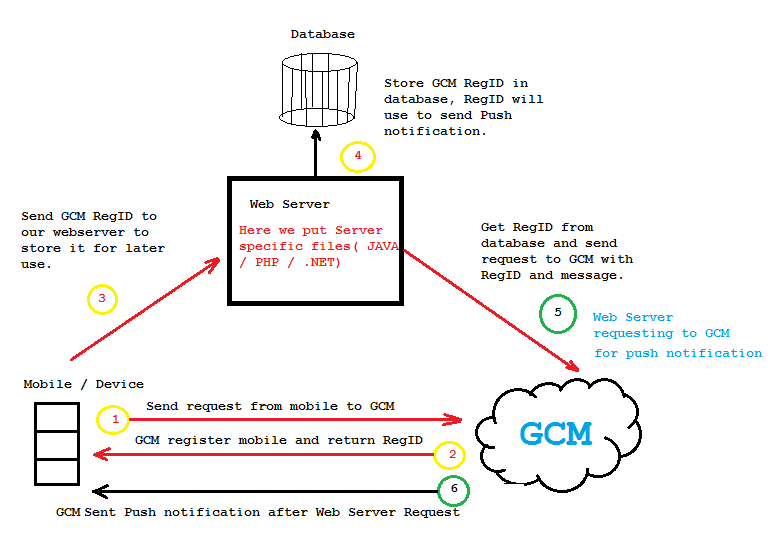
\includegraphics[scale=0.5]{image/gcm.png}
\caption{Google Cloud Messaging Working}
\end{figure}
Following are the steps to use GCM in android project:
\begin{enumerate}
\item Register with Google Cloud Messaging from GOOGLE API Console and get Sender ID and API key for Google Cloud Messaging.
\item Set Emulator for Google Cloud Messaging helper library.
\item Create Android project to register with Google Cloud Messaging(GCM).
\item Create server side code to save Google Cloud Messaging registration id in our database and send push notification to device.
\end{enumerate}

\subsubsection{HTTP Connections To Web Server}
Steps to have HTTP connection to Web Server are as follow:
\begin{enumerate}
\item Declare Internet permissions in the manifest by adding the following line to AndroidManifest.xml.
\item Create your HttpClient and HttpPost objects to execute the POST request. 
\item Set your POST data. This is done by creating and setting a list of NameValuePairs as your HttpPost's entity. Be sure to catch the UnsupportedEncodingException thrown by HttpPost.setEntity().
\item Execute the POST request. This returns an HttpResponse object, whose data can be extracted and parsed. Be sure to catch the ClientProtocolException and IOException thrown.
\end{enumerate}

\subsubsection{JSON Parsing}
JSON stands for JavaScript Object Notation.It is an independent data exchange format and is the best alternative for XML.
Steps of JSON Parsing are:
\begin{enumerate}
\item For parsing a JSON object, we will create an object of class JSONObject and specify a string containing JSON data to it. 
\item An JSON file consist of different object with different key/value pair e.t.c. So JSONObject has a seperate function for parsing each of the component of JSON file.
\end{enumerate}

\subsubsection{Broadcast Receiver}
Broadcast receiver is a component that responds to system conditions such as low battery or the screen being turned off. You can
use broadcast receivers to initiate a response from a running application, such as if a picture has been taken.
\subsubsection{Services}
Service is a process that runs in background to perform long term operations or work for remote processes. Services don't provide a User Interface.

\subsubsection{Content Provider}
It manages persistent data on the device or external sources such as web or cloud or any other system application has access to.
Android devices has on-board SQLite database management system to provide organized persistent data storage.
%%%%%%%%%%%%%%%%%%%%%%%%%%%%%%%%%%%%%%%%%%%%%%%%%%%%%%%%%%%%%%%%%
\pagebreak
\section{SnapShots of System}
Following are the snapshots of working application:
\begin{figure}[H]
\centering 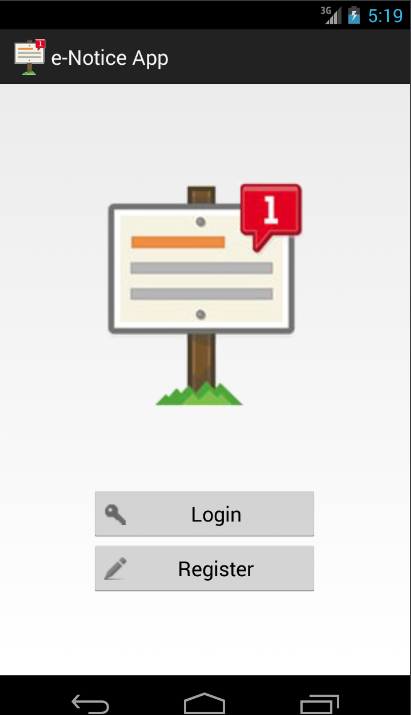
\includegraphics[scale=0.7]{image/landing.png}
\caption{Landing Page}
\end{figure}
This is the first page, the user is presented with at the first time, when he opens the application.

\begin{figure}[H]
\centering 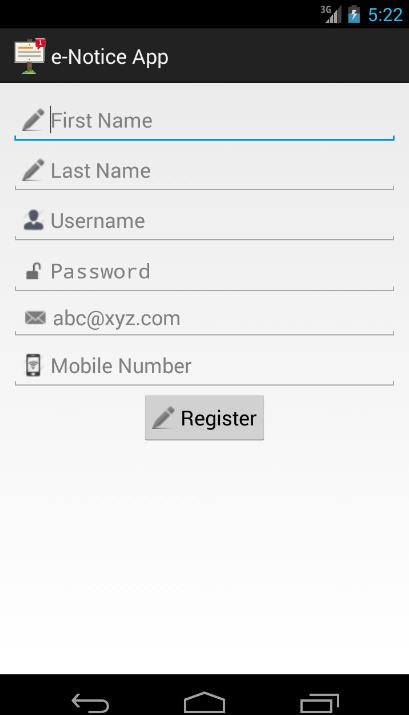
\includegraphics[scale=0.7]{image/register.png}
\caption{Register Page}
\end{figure}
This is the page where user registers himself to GCM and Web Server.

\begin{figure}[H]
\centering 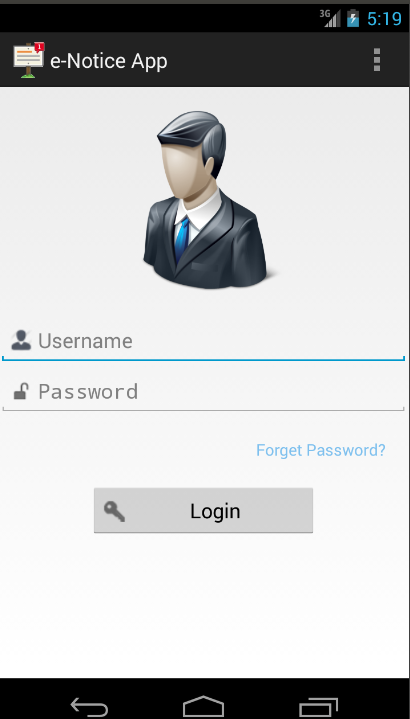
\includegraphics[scale=0.7]{image/login.png}
\caption{Login Page}
\end{figure}
This page is used to login to the application.

\begin{figure}[H]
\centering 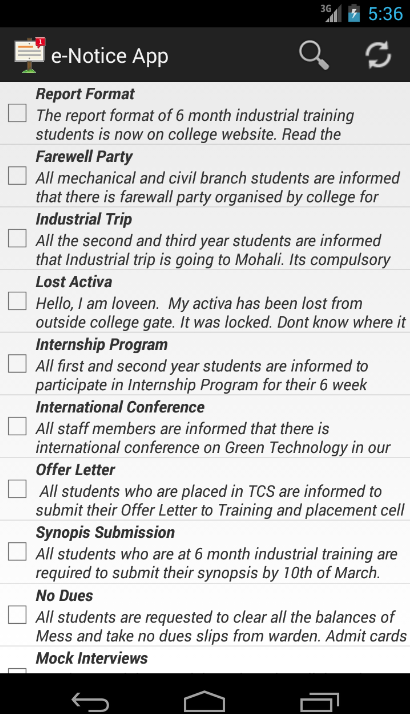
\includegraphics[scale=0.7]{image/dashboard.png}
\caption{DashBoard Page}
\end{figure}

In this page, all the notices are displayed. This is the main panel that is requierd by the normal user of application.
The user will tap on a particular notice in order to view details of notices.

\begin{figure}[H]
\centering 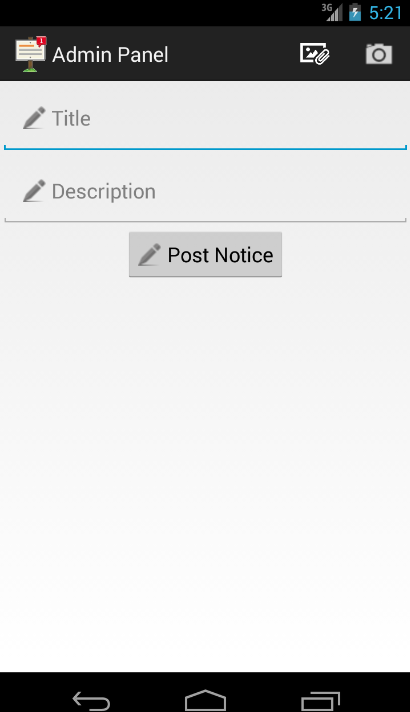
\includegraphics[scale=0.7]{image/post.png}
\caption{Post Notices Page}
\end{figure}
This is an Admin Panel Page where admin is allowed to post the message. Admin has two options of attaching image to notice.
First is to pick up image from gallery and second is to take an image from camera instantly and post with the notice.

\begin{figure}[H]
\centering 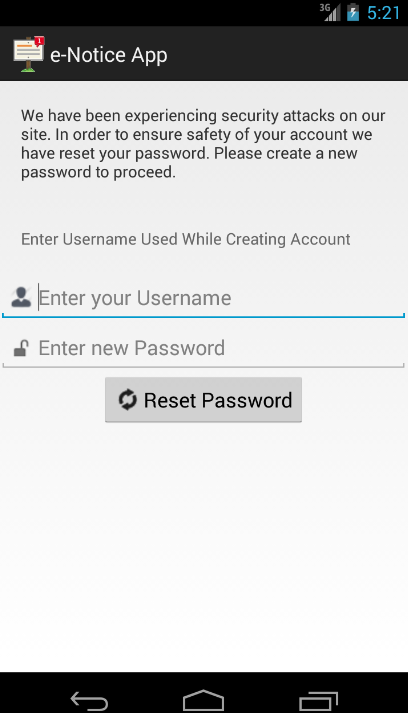
\includegraphics[scale=0.7]{image/reset.png}
\caption{Reset Password Page}
\end{figure}

This page is presented to the user when user forgots his password and want to reset the password.

\begin{figure}[H]
\centering 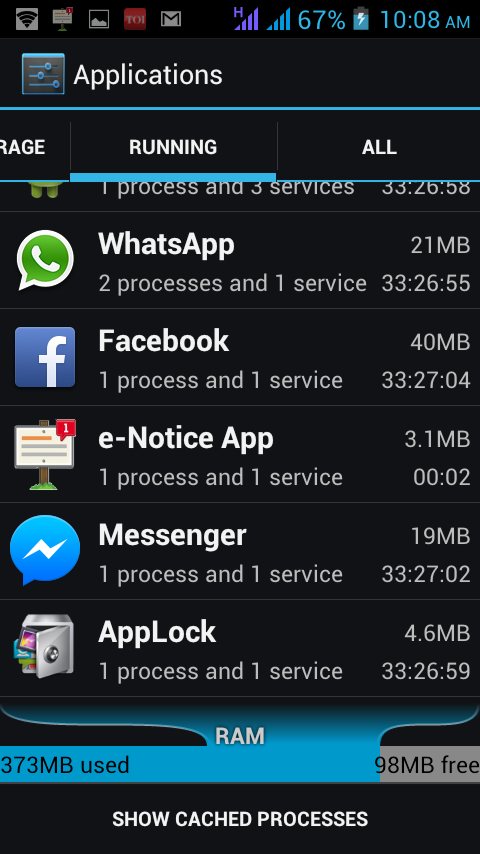
\includegraphics[scale=0.7]{image/service.png}
\caption{Intent Service Running In Application}
\end{figure}

This figure shows that service of application starts running, whenever any GCM notification arrives.

\begin{figure}[H]
\centering 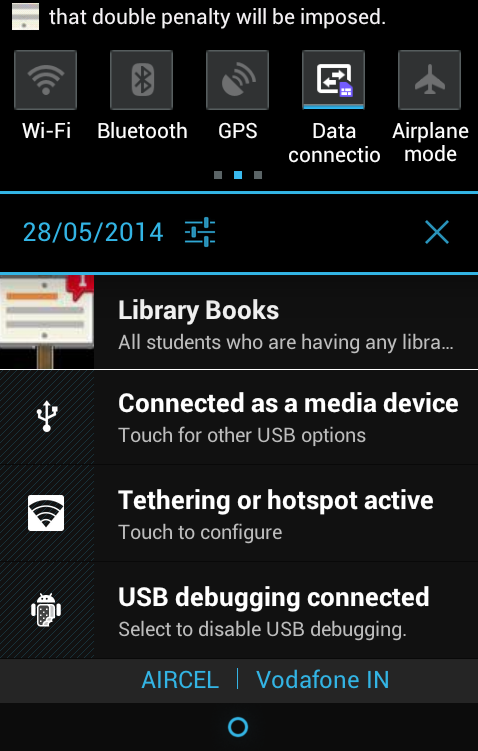
\includegraphics[scale=0.7]{image/notify.png}
\caption{Notification Received}
\end{figure}

This figure shows the notification received by the user from GCM server, whenever any notice is posted by the admin.

\begin{figure}[H]
\centering 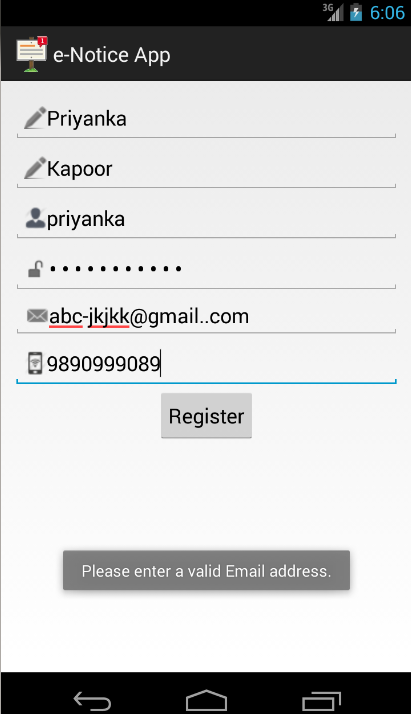
\includegraphics[scale=0.7]{image/email.png}
\caption{Email Validation}
\end{figure}

This figure shows the email validations implemented inside the application.

\begin{figure}[H]
\centering 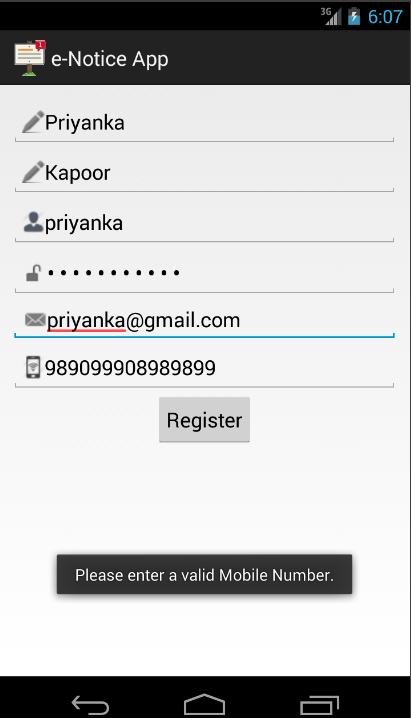
\includegraphics[scale=0.7]{image/mob.png}
\caption{Mobile Number Validation}
\end{figure}
This figure shows the mobile number validation implemented in the application.

\begin{figure}[H]
\centering 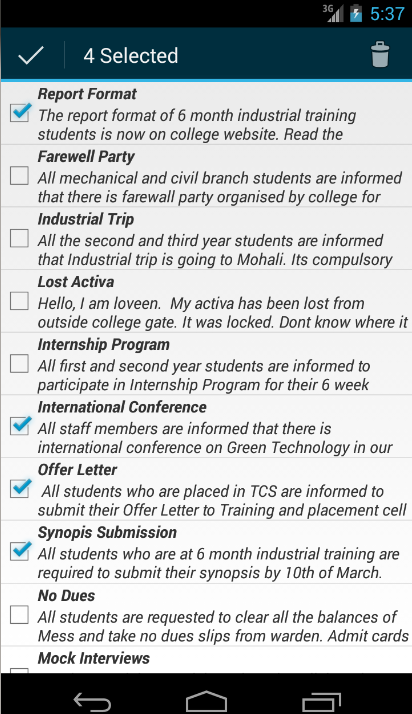
\includegraphics[scale=0.7]{image/context.png}
\caption{Contextual Action Bar}
\end{figure}
Contextual Action bar is implemented with the help of which, user is able to delete the notice.

\begin{figure}[H]
\centering 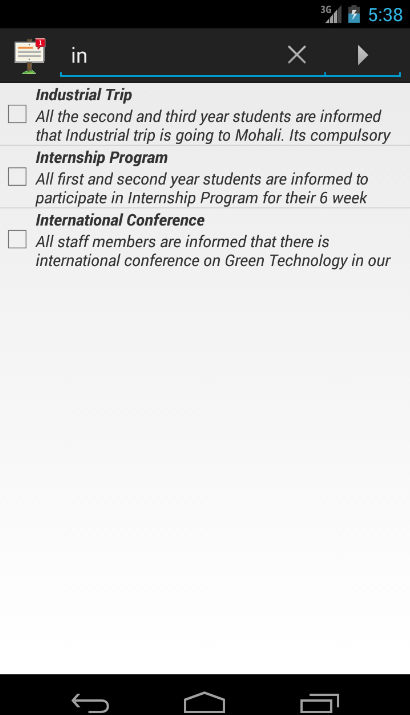
\includegraphics[scale=0.7]{image/search.png}
\caption{Search Box}
\end{figure}

This figure shows the search box available for the ease of user to search any notice by its title.

\begin{figure}[H]
\centering 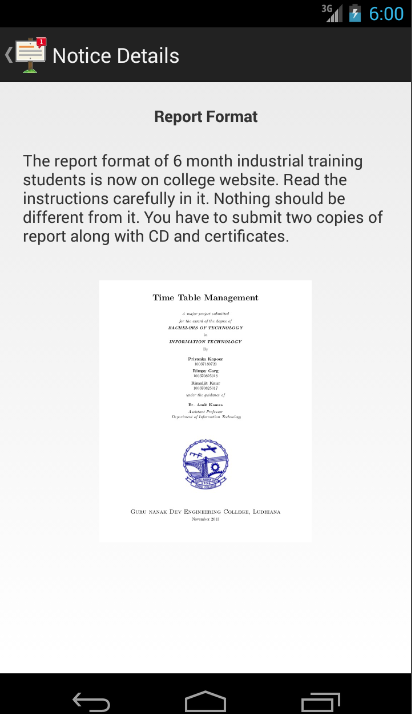
\includegraphics[scale=0.7]{image/detail.png}
\caption{Notice Details}
\end{figure}

This figure is showing the details of a particular notice that is tapped by the user.
%%%%%%%%%%%%%%%%%%%%%%%%%%%%%%%%%%%%%%%%%%%%%%%%%%%%%%%%%%%%%%%%%%%%%%%%%%%%%%%%%%%%%%%%%%%%%%%%%%%%%%%%%%%%%%%%%%%%%%%%%%%%%%%
\pagebreak
\section{Back End Representations}
The database used at the Back-end is MySQL database. Web Server used is Apache. Server side scripting language used is PHP.

Database design used at backend server has the following tables:

\begin{figure}[H]
\centering 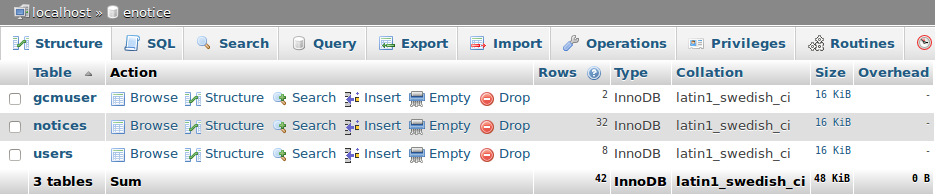
\includegraphics[scale=0.5]{image/db.png}
\caption{Tables inside Database}
\end{figure}

The first table is "gcmuser" which contains registration id given by GCM along with all personal information of the user.
The second table is "user" which just contains the id, username and password of the user.
The third table is "notices". It contains notice id, title and description of the notice, date on which the notice is posted
and filepath if a notice has an attachment.

\subsection{Snapshots of Database Tables}

\begin{figure}[H]
\centering 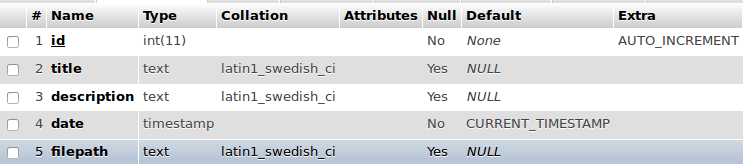
\includegraphics[scale=0.5]{image/db1.png}
\caption{Schema of GCM User Table}
\end{figure}
This table contains registration id given by GCM along with all personal information of the user like first name, last name, email id and
phone number.

\begin{figure}[H]
\centering 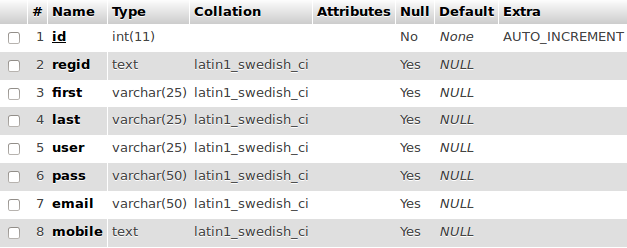
\includegraphics[scale=0.5]{image/db2.png}
\caption{Schema of User Table}
\end{figure}
This table just contains the id, username and password of the user.


\begin{figure}[H]
\centering 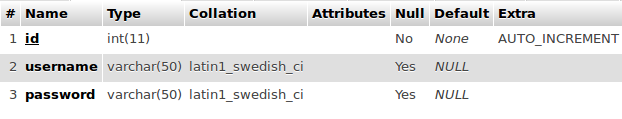
\includegraphics[scale=0.5]{image/db3.png}
\caption{Schema of Notices Table}
\end{figure}
This table contain all the details about the notices like notice id, title, description, date of notice post and filepath if the notice has an attachment.
